\subsubsection{Scopo}
Lo scopo del processo è produrre il \PPdoc , al fine di pianificare e gestire i ruoli che i membri dovranno assumere.
\subsubsection{Aspettative}
Le aspettative del processo sono:
 \begin{itemize}
  \item produrre il \PPdoc ;
  \item definire i ruoli dei membri del gruppo;
  \item definire il piano per l'esecuzione dei compiti programmati.
 \end{itemize}
\subsubsection{Descrizione}
 
\subsubsection{Ruoli di \gl{progetto}}
 In ogni momento temporale ogni membro deve ricoprire almeno un ruolo e, durante tutta la durata del progetto, ricoprire tutti i ruoli almeno una volta. Per ogni membro, le ore di lavoro devono essere il più possibile equamente distribuite. L'assegnazione e la rotazione dei ruoli sono pianificate nel \PPdocRR.
 \paragraph{Responsabile}
 Il \RESP{} è il rappresentante e il punto di riferimento del gruppo, nonché colui che si assume le responsabilità delle scelte del gruppo.
 Le responsabilità assunte sono:
 \begin{itemize}
  \item pianificazione, coordinamento e controllo delle attività;
  \item gestione delle risorse;
  \item analisi e gestione dei rischi;
  \item approvazione dei documenti;
  \item approvazione dell'offerta economica;
  \item convocazione delle riunioni interne;
  \item relazioni esterne;
  \item assegnazione delle attività a persone.
\end{itemize}
Per questi motivi ha il compito di:
\begin{itemize}
	\item assicurarsi che le attività di \gl{verifica} e \gl{validazione} siano svolte seguendo le \NPdoc;
	\item garantire il rispetto dei ruoli e dei compiti assegnati nel \PPdoc.
\end{itemize}
 \paragraph{Amministratore}
 L'\AMM{} è responsabile dell'efficienza dell'ambiente di lavoro, in particolare si occupa di:
 \begin{itemize}
  \item studiare e fornire strumenti che migliorano l'ambiente di lavoro, automatizzando il lavoro ove possibile;
  \item gestire archiviazione, versionamento e configurazione dei documenti e del \gl{software};
  \item garantire la qualità del \gl{prodotto}, fornendo procedure e strumenti di monitoraggio e segnalazione;
  \item eliminare le difficoltà sulla gestione di processi e risorse.
 \end{itemize}
 L'\AMM{} non compie scelte gestionali, ma tecnologiche concordate con il \RESP.
 \paragraph{Analista}
 L'\AN{} deve identificare e comprendere il dominio del problema. \\
 In particolare si occupa di:
 \begin{itemize}
  \item mappare le richieste del cliente in specifiche per il prodotto;
  \item catalogare e spiegare specifiche comprensibili nell'\ARdoc{} e nello \SFdoc{};
  \item classificare i requisiti;
  \item stendere i diagrammi dei \gl{casi d'uso};
  \item assegnare i requisiti a parti distinte del \gl{sistema};
  \item assicurarsi che i requisiti trovati siano conformi alle richieste del \gl{proponente};
  \item definire test di sistema e di accettazione al fine di verificare i requisiti.
\end{itemize}
L'\AN{} non si occupa di trovare una soluzione al problema, ma lo definisce redigendo lo \textit{"Studio di Fattibilità"} e l'\textit{"Analisi dei Requisiti"}. 

 \paragraph{Progettista}
 Il \PJ{} ha forti competenze sullo \gl{stack} tecnologico usato. \\
 In particolare deve: 
 \begin{itemize}
  \item indicare le tecnologie più adatte allo sviluppo del progetto;
  \item descrivere il funzionamento del sistema progettandone l'architettura;
  \item produrre una soluzione fattibile in termini di risorse.
 \end{itemize}
Il \PJ{} redige i documenti di \textit{"Specifica Tecnica"}, \textit{"Definizione di prodotto"} e si occupa delle sezioni del \textit{"Piano di Qualifica"} relative alle metriche di verifica della programmazione.

\paragraph{Programmatore}
 Il \PR{} si occupa della codifica, in particolare:
 \begin{itemize}
  \item implementa le soluzioni indicate dal \PJ ;
  \item scrive codice documentato, versionato e mantenibile nel rispetto delle \NPdoc ;
  \item realizza e fornisce gli strumenti per verificare e validare il prodotto.
 \end{itemize}
 \paragraph{Verificatore}
 Il \VER , disponendo di una profonda conoscenza delle \NPdoc , si occupa delle attività di verifica. \\
 In particolare deve: 
 \begin{itemize}
  \item controllare il rispetto delle \NPdoc durante ogni attività del progetto.
 \end{itemize}
 \paragraph{Rotazione dei ruoli}
 Ogni membro del gruppo dovrà ricoprire ciascuno dei ruoli del progetto. La pianificazione dovrà essere redatta prestando attenzione a quanto segue:
 \begin{itemize}
 	\item ogni membro del gruppo non dovrà mai ricoprire un ruolo che preveda la verifica dell'operato svolto da lui in precedenza poiché questo potrebbe portare ad un conflitto di interesse;
 	\item bisogna tener conto dei possibili impegni o interessi dei singoli membri del gruppo;
 	\item ciascun membro dovrà assicurare l'esclusivo svolgimento del ruolo a lui assegnato.
 \end{itemize}  
\subsubsection{Comunicazioni}
 \paragraph{Interne}
 È stato creato un gruppo Telegram, accessibile solo ai membri del \gl{team}, per effettuare le comunicazioni interne. In caso siano necessaria maggiore interazione, si farà utilizzo di \gl{Google Hangouts}. 
 \paragraph{Esterne}
 È stata creata un'apposita cartella di posta elettronica per mantenere i contatti con il proponente, il committente ed altre eventuali figure esterne.\\
  Inoltre, su richiesta dell'azienda proponente \PROPONENTE, è stato creato un apposito dominio \gl{Slack} per permettere una veloce interazione tra i gruppi fornitori e l'azienda. Il dominio è zero12university. \\
 La gestione della casella di posta elettronica e di Slack è compito del \RESP. \\
 L'indirizzo e-mail è il seguente: \EMAIL.
 \paragraph{Email}
 Le mail devono essere scritte nella maniera più chiara e corretta possibile, in particolare ognuna di esse deve essere composta di:
 \begin{itemize}
 	\item destinatario;
 	\item oggetto, che deve essere breve e diretto;
	\item contenuto, che deve essere chiaro ed esaustivo;
	\item firma del responsabile.
 \end{itemize}
 Nel caso si vogliano scambiare dei documenti, si deve a evitare l'invio di allegati tramite email e preferire l'utilizzo di un apposito sito di scambi, quale ad esempio Google Drive.
\subsubsection{Incontri}
 \paragraph{Interni}
 Ogni membro del team può proporre un incontro interno tramite il \gl{bot} Telegram \gl{VotePoll}, specificando i motivi e l'oggetto dell'incontro. 
 Sarà poi compito del \RESP{} decidere se effettuare l'incontro o meno.\\
  La verbalizzazione degli incontri interni è compito di uno tra gli \AMMP.
 \paragraph{Esterni} 
 Ogni membro del team può proporre un incontro esterno tramite il bot Telegram VotePoll, specificando i motivi e l'oggetto dell'incontro. 
Se il \RESP{} decide che l'incontro può essere organizzato dovrà accordarsi con la figura esterna, e comunicare gli estremi della riunione ai membri del team.\\
 La verbalizzazione degli incontri esterni è compito del \RESP.
 \paragraph{Gestione}
 All’inizio di ogni riunione interna il \RESP{} nomina l'amministratore che ha il compito di tracciare gli aspetti più importanti della riunione, con lo scopo di esporli poi nel relativo verbale. Questo verbale verrà archiviato nel repository del gruppo, in modo da permetterne la consultazione. Se invece la riunione è esterna, questo compito è delegato al \RESP{}.
 Durante le riunioni i partecipanti devono tenere un comportamento che favorisca la discussione all’interno del gruppo.
 
\subsubsection{Strumenti di coordinamento}
 \paragraph{\gl{Ticketing}}
 Il \RESP{} ha il compito di assegnare i \gl{task} ai membri del team utilizzando l'applicativo web \gl{Asana}. \\
 Definendo delle \gl{milestone}, è possibile tenere traccia dello stato di avanzamento del lavoro di ogni task.
 
 \subsubsection{Rischi}
 Il \RESP{} ha il dovere di individuare e monitorare i rischi indicati nel \PPdoc. In caso ne vengano identificati di nuovi, il \RESP{} deve agire nel modo seguente:
 \begin{itemize}
  \item comunicare i nuovi rischi al team;
  \item pianificare una strategia per la gestione dei nuovi rischi;
  \item aggiornare le procedure di gestione dei rischi nel \PPdoc.
 \end{itemize}
 \subsubsection{Procedure}
 \paragraph{Richiesta riunione interna}
 Per chiedere una riunione interna, si deve seguire la seguente procedura:
 \begin{itemize}
 	\item effettuare l'accesso in Telegram;
 	\item selezionare la chat "VoteBot";
 	\item inserire in un solo messaggio:
 	\begin{itemize}
 		\item oggetto della riunione;
 		\item contenuto da affrontare;
	 	\item giorno proposto;
	 	\item dare "Invio";
 	\end{itemize}
 	\item inserire le opzioni di voto, le quali dovranno essere gli orari nei quali si propone di fare la riunione.
 	\item selezionare "Publish Poll";
 	\item selezionare la chat del gruppo.
 \end{itemize}
 Una volta che tutti hanno votato, il \RESP{} provvederà ad approvare la proposta o meno.
 \paragraph{Richiesta riunione esterna}
 Per chiedere una riunione esterna, si deve seguire la seguente procedura:
 \begin{itemize}
 	\item effettuare l'accesso in Telegram;
 	\item selezionare la chat "VoteBot";
 	\item inserire in un solo messaggio:
 	\begin{itemize}
 		\item oggetto della riunione;
 		\item contenuto da affrontare;
 		\item giorno proposto;
 		\item dare "Invio";
 	\end{itemize}
 	\item inserire le opzioni di voto, le quali dovranno essere gli orari nei quali si propone di fare la riunione.
 	\item selezionare "Publish Poll";
 	\item selezionare la chat del gruppo.
 \end{itemize}
 Una volta che tutti hanno votato, il \RESP{} provvederà ad approvare la proposta o meno. \\
 Se approvata, il \RESP{} provvederà a comunicare all'entità esterna gli estremi della riunione che il gruppo propone. In caso l'entità esterna proponga altri estremi, il \RESP{} dovrà informare i membri del gruppo, al fine di decidere la fattibilità della proposta. 
 \paragraph{Gestione dei ticket}
 \subparagraph{Creazione}
Per creare un task viene utilizzato l'applicativo web Asana. Per ogni task viene creato un progetto separato rispetto al progetto \PROGETTO{}, col nome del task da eseguire. Tale progetto viene diviso in una serie di sottocompiti i quali verranno scritti come task sulla "bacheca" del
progetto, senza essere ancora assegnati a nessuno.
 \subparagraph{Assegnazione}
 Per l'assegnazione dei task i membri del progetto si occuperanno
di prendere un task a testa e di portarlo a termine, assegnandolo a sè stessi. Ogni
volta che un membro porta a termine un task, ne prende un altro. I task
saranno decisi dal responsabile in carica alla creazione del progetto, il quale
dovrà anche controllare l'assegnazione dei compiti. A tale scopo,
il responsabile sarà iscritto a tutti i compiti di tutti i progetti con l'account del gruppo,
per facilitare il passaggio da un responsabile al successivo.
\subsubsection{Strumenti}
 \paragraph{Telegram}
 Telegram è un software libero che fornisce un servizio di messaggistica istantanea erogato senza fini di lucro dalla società Telegram LLC. È stato ritenuto più adatto di Whatsapp.
 \paragraph{Google Hangouts}
 Hangouts è un software di messaggistica istantanea e di \gl{VoIP}   sviluppato da Google. È disponibile per le piattaforme mobili \gl{Android} e \gl{iOS} e come estensione per il \gl{browser} web Google Chrome. Inoltre, permette la condivisione degli schermi tra i membri della chiamata. È stato ritenuto più adatto di Skype.
 \paragraph{Google Drive}
 Google Drive è un applicativo web che consente lo scambio di file tra più persone. Il gruppo \GRUPPO dovrà far utilizzo di questo strumento per lo scambio di file con le entità esterne.
 \paragraph{Asana}
 Asana è un applicativo web e mobile che consente al team di assegnare, tracciare e gestire dei task.
\begin{figure}[h]
\centering
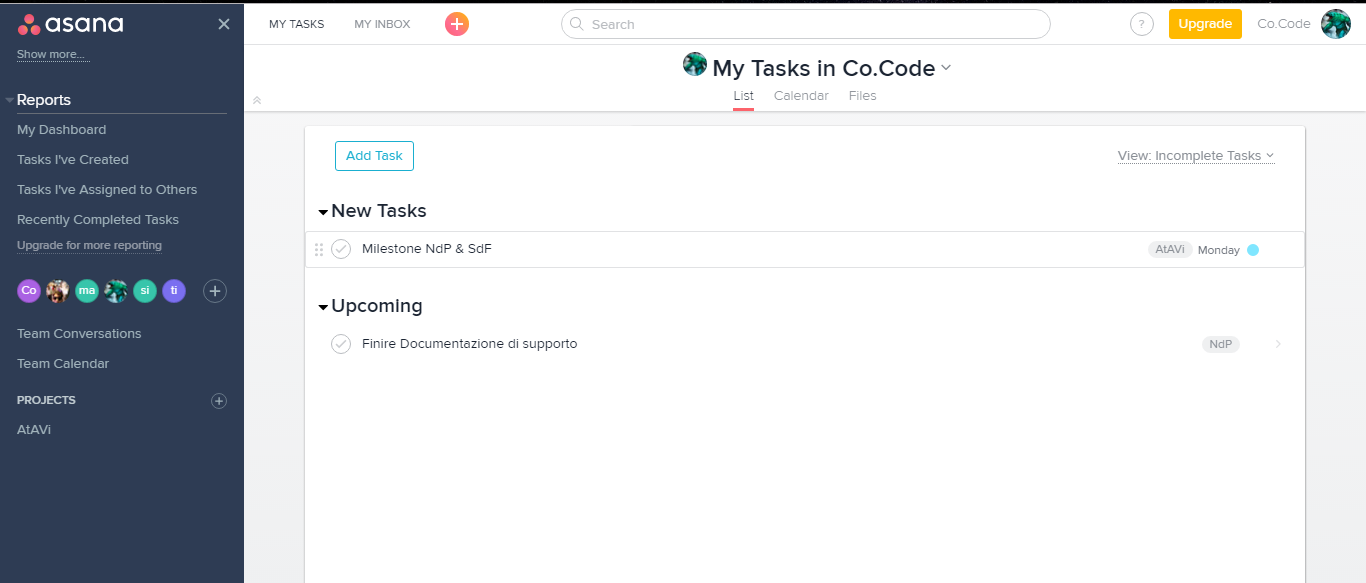
\includegraphics[scale=0.4]{img/asana.png}
\caption{Asana}\label{sec:Figura5}
\end{figure}
 \paragraph{GanttProject} 
 GanttProject è un software gratuito per la creazione di grafici rappresentanti l'organizzazione e gestione di compiti e milestone all'interno di un progetto. Verrà utilizzato nella versione 2.7 o superiore.
\begin{figure}[h]
\centering
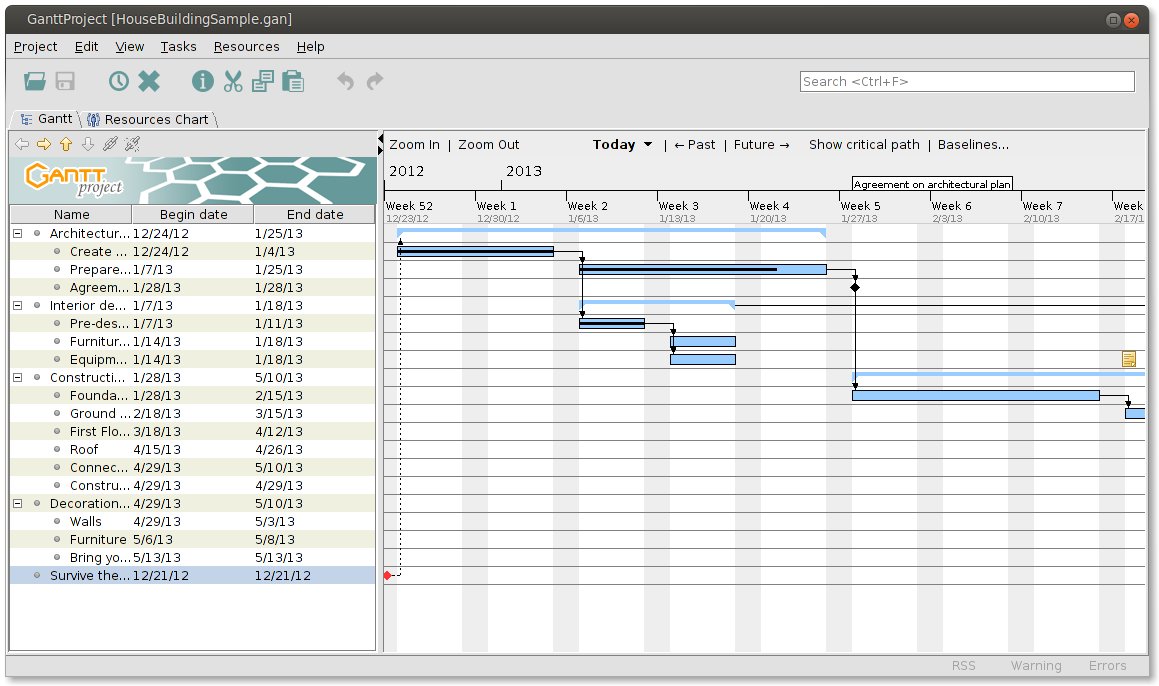
\includegraphics[scale=0.35]{img/gantt.png}
\caption{GanttProject}\label{sec:Figura6}
\end{figure} 